\documentclass[preprint]{sig-alternate}

\usepackage{cite}
\usepackage{graphicx}
\usepackage{algorithm,algpseudocode}
\usepackage{algorithmicx}


\usepackage{amssymb}
\usepackage{mathrsfs}
\usepackage{amsmath}


\usepackage[sans]{dsfont}
\usepackage{stmaryrd}
\usepackage{pifont}
\usepackage{wasysym}

\usepackage{array}
\usepackage{url}
\usepackage[usenames]{color}
\usepackage[tight,footnotesize]{subfigure}



\renewcommand{\algorithmicrequire}{\textbf{Input:}}
\renewcommand{\algorithmicensure}{\textbf{Output:}}

\newtheorem{example}{Example}
\newtheorem{definition}{Definition}
\newtheorem{conjecture}{Conjecture}
\newtheorem{lemma}{Lemma}
\newtheorem{theorem}{Theorem}
\newtheorem{corollary}[theorem]{Corollary}
\newtheorem{proposition}[theorem]{Proposition}
\def\endexam{\hspace*{\fill}~$\diamond$\par\endtrivlist\unskip}

\setlength{\pdfpagewidth}{8.5in}
\setlength{\pdfpageheight}{11in}



\begin{document}


\title{Improving Building Energy Efficiency by Kinect-based Occupancy
  Tracking and Mobility Detection System}

\numberofauthors{1}
\author{\alignauthor  \ \\
\affaddr{some authors} \\
%\email{%\{\}@masdar.ac.ae}
}


\makeatletter
\let\@copyrightspace\relax
\makeatother

\pagestyle{plain}
\thispagestyle{plain}

\maketitle


\begin{abstract}
In an average open office building, air conditioning, ventilation and
lighting account for 30 to 40 percent of energy consumption. Nowadays,
most modern air conditioning systems in buildings still operate based on
pre-assumed occupancy schedule rather than actual usage. Such operation mode creates
needless conditioning and energy waste. Therefore, in order to achieve
an optimal conditioning state based on  traffic in zones of interest,
we need to know the rate and time of occupancy and intelligently tune
the system according to the number of actual occupants. In our
study, we use a people counting software based on a network of
Microsoft Kinect for Windows sensors in order to acquire temporal
occupancy information. The occupancy counting software provides
real-time occupancy data through detection and tracking of people in
the building.  An HVAC management and control system needs to adjust
this data in real-time and measure the local level of comfort. In
this research, we propose an approach for energy saving which
integrates a real-time occupancy data into building management
systems. This approach leads us to the creation of an occupancy
monitoring and control system which takes into account three elements:
subject mobility, room status (e.g.\ empty, occupied, crowded) and
actual number of people.  In addition, in order to model the occupancy
data collected, we use the Markov Chain principle where a state is a
combination of the statuses of existing zones in the building. Such
state represents the level of energy consumption in real time and a
useful input data for the HVAC system controller.  Here, we
demonstrate that our model, based on data collected by an ensemble of
Kinect sensors, can be integrated with an HVAC control strategy to
achieve substantial energy savings. Through the prediction of future
occupancy level of particular zones of a building, our intelligent
system is able to adjust conditioning parameters gradually to reflect
the predicted changes in time. 


% A little bit noisy at lab. Who could possibly help me figure out how
% and why...
\end{abstract}


\noindent
{\bf Categories and Subjects:} {[Computer systems organization]}: {\em Embedded and cyber-physical systems}: {\em Sensors and actuators}

\noindent
{\bf General Terms: }Algorithms, Design, Management


\noindent
{\bf Keywords: }Wireless Sensor Networks,
\\

\section{Introduction}
\label{sec:intro}

A 2009 report by the United Nations Environment Program (UNEP SBCI)
\cite{huovila2009buildings} has clearly identified  construction
buildings as responsible of a significant amount of global energy use
and greenhouse gas emissions in both developed and developing
countries. Although most local governments have taken steps through
regulations and policies to reduce energy use and gas emissions, their
efforts have had little impact in the past. In addition,  these
measures are likely to meet some resistance in the future because they
may not serve the economic interests of the many stakeholders involved
in the building sector. Therefore,  there is a need for an innovative
system that implements energy efficiency measures. Such system would
provide locally small energy-reduction opportunities for each of the
millions of buildings across the globe.

At the core of energy consumption in buildings, are Heat Ventilation
And Cooling systems (HVAC) which are mostly designed to operate at
full capacity under the assumption of normal occupancy of rooms at all
time. Although current HVAC systems are equipped with sensors, their
management and control systems ignore the dynamic nature of daily
occupancy of buildings. In addition, they are unable to proactive
adjust to occupants' comfort levels. Understanding	human mobility
and occupancy patterns are key factors in successfully managing energy
in buildings. Building occupancy has been the subject of intensive
studies in the past years. Several approaches using building occupancy
data to improve prediction and simulation of HVAC control have been
proposed. In the same perspective, the main objective of our paper is
to propose an energy-saving model based on occupancy patterns of human
mobility in buildings. This model offers a solution for the management
and control of HVAC systems in smart buildings. The most important
features of the system that implements this model are the following:

\begin{enumerate}
\item  The {\em detection and tracking of people in real time} in the
  building provides accurate occupancy data of an entire building
  divided into several related zones.
\item  A  {\em Occupancy Counter Software} carries out the detection,
  tracking and monitoring process based on multiple Microsoft Kinect
  for Windows (K4W) sensors distributed in strategic locations in the
  building.
\item A {\em prediction of future occupancy} of the building is
  introduced through the use of a Markov chain (MC) which models the
  collected occupancy data.  MC is a suitable because it captures the
  temporal nature of occupancy variation along with inter-room
  correlations and occupant usage.  Unlike most building occupancy
  techniques described in the Related works
  Section~\ref{sec:relatedworks}, our approach implements an occupancy
  counting technique that is based on the Microsoft Kinect for Windows
  (K4W) device.
\end{enumerate}

{\bf Organization:}This paper is organized as follows: In
Section~\ref{sec:background}, we present relevant background
information about human detection and tracking techniques and tools as
well as the most popular occupancy counting and sensing devices. In
particular, we mention the Microsoft Kinect for Windows that is
central to our experimentation. Next, in Section~\ref{sec:design}, we
discuss about the design and implementation of our solution to
energy-saving problem in smart buildings.  Here, we give a detailed
account of the setup of our human mobility tracking and detection
system based on a occupancy counter software using the Kincet for
windows sensor. In Section~\ref{sec:relatedworks}, we expose several
approaches using building occupancy data to improve prediction and
simulation of HVAC control. These approaches use models or techniques
that are related  to our study. Then, in Section~\ref{sec:evaluation},
we displays the results and evaluations of our real world test-bed
conducted in an open office laboratory.  In
Section~\ref{sec:conclusion}, we conclude our paper and propose some
perspectives. 


\section{Background}
\label{sec:background}


This section presents background information on human detection	and tracking approaches and related techniques as well as the most popular sensing devices. In  particular, it gives a brief description of the Microsoft Kinect for Windows (K4W) sensor.  In addition, we give an overall picture of the methods and counting logic useful to our occupancy counter software.

\subsection{Human Detection and Tracking}
Human detection and tracking (HDT) is an active research subfield of object recognition. Detecting the presence of humans in a particular environment and planing resources accordingly are at the core of many problem-solving strategies in construction management. Human motion tracking includes capturing body displacements and limb movements such as postures and gestures of human targets. These strategies should be able to predict through a learning mechanism, an acceptable number of occupants of a room  \cite{realtimepeoplecount}. Such prediction is important in overcoming the necessary time delay between signal detection and appropriate temperature.

\subsubsection{Approaches in HDT}
HDT is by nature a complex process that includes issues as simple as adequate sensing to the delicate data-mining techniques. It is a challenging task for a number of reasons. The common obstacles to quality detection and tracking are ambient noise, device imperfection, environmental factors variation, fluctuation of data collected, background signal similarity and sometimes, intentional deception (adversarial scenario). Our interest in this study is limited to the well known spatio-temporal properties related to the position and history (tracks) of human present in a given environment. These properties are presence, count, location, track and identity.

\subsubsection{Sensor Technologies for HDT}
Several kinds of counters that require contact with people, such as turnstiles, are used because contact type counters count very accurately. These counters, however, cannot be applied to spaces within commercial buildings because, except at a few critical places (e. g. , entrances), they obstruct the normal flow of people in work spaces and would require installation in each room \cite{Yoshinaga}. Several kinds of sensors currently can provide information on occupancy, such as video cameras equipped with occupancy counting software, optical tripwires and pyroelectric infrared (PIR) motion sensors that count the number of people crossing a particular area. Wireless sensor networks have been widely used as supported technologies for monitoring, tracking and controlling Human Mobility. Most of studies designed a WSN for occupancy detection and result data analysis to send a final control function to the thermostat for HVAC monitoring. The authors of \cite{TinyAgent} highlighted another approach in occupancy detection by using sensors called Tiny Agents (TA) to control power consumption in a building. The tiny agents are distributed throughout the building and deployed in air-conditioning system to capture and send room temperatures and interact with the AC or other agents.

\subsubsection{Occupancy Counters}
An Occupancy Counter is a system that counts the number of persons entering and exiting a room. Many devices based on several technologies (ex. Cameras, infrared beams, vision) have been used with various level of success in commercial systems to count people indoor and outdoor.Remarkable research using 1) neural networks to count subjects in video images and 2) algorithms that use single or multiple lines as counting zones  have also been proposed.

\subsection{The Microsoft Kinect Sensor}
 The Kinect sensor is a motion sensing device with an infrared depth sensor , an emitter and a microphone sound system built around an maleable RGB camera as shown in Figure \ref{fig:kcom}.  Kinect array specification include  a 43 degrees vertical angle viewing  and 57 horizontal degrees  of field of view. This is a motion sensing input that enables a user to remote control a host system via gesture and sound commands. Optical and acoustical detections are the motion sensing that can be electronically identified. Infrared light or laser technology may be used for optical detection because Kinect is an electronic sensor. The Kinect sensor also performs functions such as voice recognition, facial recognition, and skeletal tracking along with motion detection \cite{aboutkinect}. The depth camera, a virtual camera, is the result of displacement matching on the IR projector and real IR camera, each equipped with its own lens distortion.  The depth data from Kinect sensor is the distance, in millimeters, to the nearest object at that particular (x, y) coordinate in the depth sensor’s field of view.

\begin{figure} [!ht]
  \begin{center}
	  	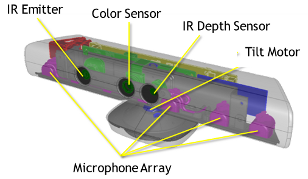
\includegraphics[width=0.9\columnwidth]{./images/k4w350.png}
  \end{center}
  \caption{Kinect component}\label{fig:kcom}
\end{figure}

There are a variety of open source libraries for Kinect programming using PC's like libfreenect, openni and SDK. Open Kinect \cite{openkinect} is community of people who use libfreenect, a free and open source library for enabling Kinect programming in PC’s run by Windows, Linux, and Mac. Open-Kinect support many wrappers like python, c++, c]. The official library from Microsoft Kinect SDK  provides features like color images, depth images, audio input, and skeletal data. The tracking mechanism in software technology used in Kinect enables advanced gesture, facial and voice recognitions.




\bibliographystyle{plain}
\bibliography{reference}


\end{document}

